\documentclass{standalone}
\usepackage{tikz}
\usetikzlibrary{patterns, positioning}


\begin{document}
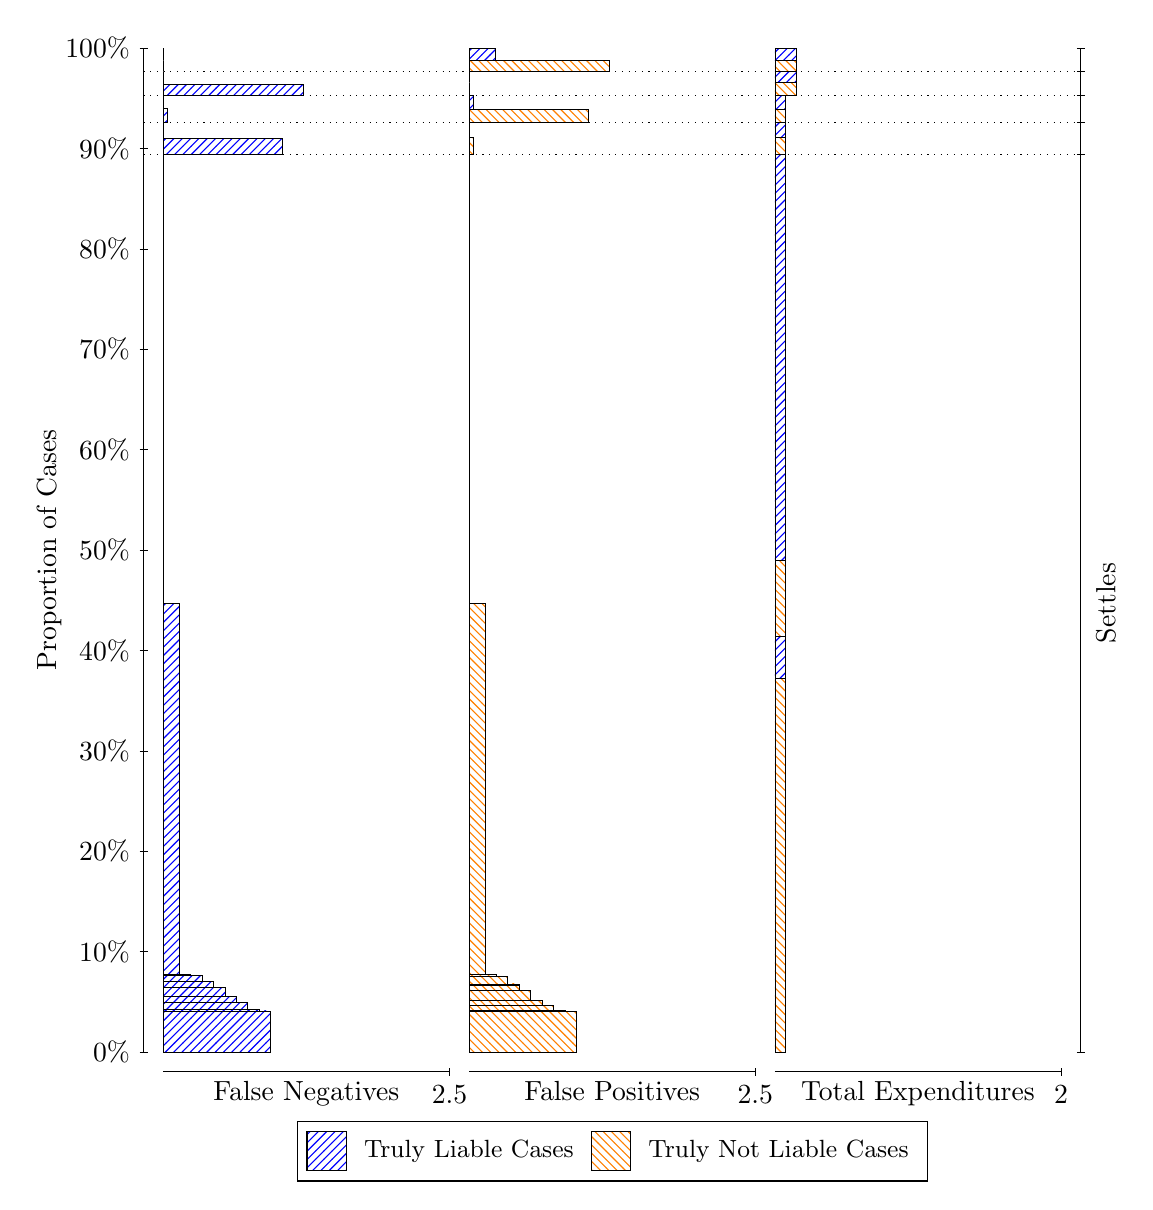
\begin{tikzpicture}
\draw[black, very thin] (1.5,1.75) -- (1.5,14.5);
\node[rotate=90, text=black, anchor=center] at (0.3, 8.125) {Proportion of Cases};
\draw[black, very thin] (1.45,1.75) -- (1.55,1.75);
\node[text=black, anchor=east] at (1.45, 1.75) {0\%};
\draw[black, very thin] (1.45,3.025) -- (1.55,3.025);
\node[text=black, anchor=east] at (1.45, 3.025) {10\%};
\draw[black, very thin] (1.45,4.3) -- (1.55,4.3);
\node[text=black, anchor=east] at (1.45, 4.3) {20\%};
\draw[black, very thin] (1.45,5.575) -- (1.55,5.575);
\node[text=black, anchor=east] at (1.45, 5.575) {30\%};
\draw[black, very thin] (1.45,6.85) -- (1.55,6.85);
\node[text=black, anchor=east] at (1.45, 6.85) {40\%};
\draw[black, very thin] (1.45,8.125) -- (1.55,8.125);
\node[text=black, anchor=east] at (1.45, 8.125) {50\%};
\draw[black, very thin] (1.45,9.4) -- (1.55,9.4);
\node[text=black, anchor=east] at (1.45, 9.4) {60\%};
\draw[black, very thin] (1.45,10.675) -- (1.55,10.675);
\node[text=black, anchor=east] at (1.45, 10.675) {70\%};
\draw[black, very thin] (1.45,11.95) -- (1.55,11.95);
\node[text=black, anchor=east] at (1.45, 11.95) {80\%};
\draw[black, very thin] (1.45,13.225) -- (1.55,13.225);
\node[text=black, anchor=east] at (1.45, 13.225) {90\%};
\draw[black, very thin] (1.45,14.5) -- (1.55,14.5);
\node[text=black, anchor=east] at (1.45, 14.5) {100\%};

\draw[black, very thin] (13.4,1.75) -- (13.4,14.5);
\draw[black, very thin] (13.35,1.75) -- (13.45,1.75);
\node[anchor=west] at (13.35, 1.75) {};
\draw[black, very thin] (13.35,13.153) -- (13.45,13.153);
\node[anchor=west] at (13.35, 13.153) {};
\draw[black, very thin] (13.35,13.557) -- (13.45,13.557);
\node[anchor=west] at (13.35, 13.557) {};
\draw[black, very thin] (13.35,13.901) -- (13.45,13.901);
\node[anchor=west] at (13.35, 13.901) {};
\draw[black, very thin] (13.35,14.199) -- (13.45,14.199);
\node[anchor=west] at (13.35, 14.199) {};
\draw[black, very thin] (13.35,14.5) -- (13.45,14.5);
\node[anchor=west] at (13.35, 14.5) {};

\draw[black, very thin, pattern color=blue, pattern=north east lines] (1.75,1.75) rectangle (3.1125,2.2728);
\draw[black, very thin, pattern color=blue, pattern=north east lines] (1.75,2.2728) rectangle (2.9672,2.288);
\draw[black, very thin, pattern color=blue, pattern=north east lines] (1.75,2.288) rectangle (2.8218,2.3757);
\draw[black, very thin, pattern color=blue, pattern=north east lines] (1.75,2.3757) rectangle (2.6765,2.4532);
\draw[black, very thin, pattern color=blue, pattern=north east lines] (1.75,2.4532) rectangle (2.5312,2.5743);
\draw[black, very thin, pattern color=blue, pattern=north east lines] (1.75,2.5743) rectangle (2.3858,2.651);
\draw[black, very thin, pattern color=blue, pattern=north east lines] (1.75,2.651) rectangle (2.2405,2.7193);
\draw[black, very thin, pattern color=blue, pattern=north east lines] (1.75,2.7193) rectangle (2.0952,2.7391);
\draw[black, very thin, pattern color=blue, pattern=north east lines] (1.75,2.7391) rectangle (1.9498,7.4513);
\draw[black, very thin, pattern color=orange, pattern=north west lines] (1.75,7.4513) rectangle (1.75,13.153);
\draw[black, very thin, pattern color=blue, pattern=north east lines] (1.75,13.153) rectangle (3.2578,13.348);
\draw[black, very thin, pattern color=orange, pattern=north west lines] (1.75,13.348) rectangle (1.75,13.557);
\draw[black, very thin, pattern color=blue, pattern=north east lines] (1.75,13.557) rectangle (1.8045,13.736);
\draw[black, very thin, pattern color=orange, pattern=north west lines] (1.75,13.736) rectangle (1.75,13.901);
\draw[black, very thin, pattern color=blue, pattern=north east lines] (1.75,13.901) rectangle (3.5303,14.04);
\draw[black, very thin, pattern color=orange, pattern=north west lines] (1.75,14.04) rectangle (1.75,14.199);
\draw[black, very thin, pattern color=orange, pattern=north west lines] (1.75,14.199) rectangle (1.75,14.339);
\draw[black, very thin, pattern color=blue, pattern=north east lines] (1.75,14.339) rectangle (1.75,14.5);
\draw[black, very thin, pattern color=orange, pattern=north west lines] (5.6333,1.75) rectangle (6.9958,2.2702);
\draw[black, very thin, pattern color=orange, pattern=north west lines] (5.6333,2.2702) rectangle (6.8505,2.2821);
\draw[black, very thin, pattern color=orange, pattern=north west lines] (5.6333,2.2821) rectangle (6.7052,2.3411);
\draw[black, very thin, pattern color=orange, pattern=north west lines] (5.6333,2.3411) rectangle (6.5598,2.4079);
\draw[black, very thin, pattern color=orange, pattern=north west lines] (5.6333,2.4079) rectangle (6.4145,2.5289);
\draw[black, very thin, pattern color=orange, pattern=north west lines] (5.6333,2.5289) rectangle (6.2692,2.5951);
\draw[black, very thin, pattern color=orange, pattern=north west lines] (5.6333,2.5951) rectangle (6.2692,2.6138);
\draw[black, very thin, pattern color=orange, pattern=north west lines] (5.6333,2.6138) rectangle (6.1238,2.7103);
\draw[black, very thin, pattern color=orange, pattern=north west lines] (5.6333,2.7103) rectangle (5.9785,2.7352);
\draw[black, very thin, pattern color=orange, pattern=north west lines] (5.6333,2.7352) rectangle (5.8332,7.4514);
\draw[black, very thin, pattern color=blue, pattern=north east lines] (5.6333,7.4514) rectangle (5.6333,13.153);
\draw[black, very thin, pattern color=orange, pattern=north west lines] (5.6333,13.153) rectangle (5.6878,13.363);
\draw[black, very thin, pattern color=blue, pattern=north east lines] (5.6333,13.363) rectangle (5.6333,13.557);
\draw[black, very thin, pattern color=orange, pattern=north west lines] (5.6333,13.557) rectangle (7.1412,13.723);
\draw[black, very thin, pattern color=blue, pattern=north east lines] (5.6333,13.723) rectangle (5.6878,13.901);
\draw[black, very thin, pattern color=orange, pattern=north west lines] (5.6333,13.901) rectangle (5.6333,14.06);
\draw[black, very thin, pattern color=blue, pattern=north east lines] (5.6333,14.06) rectangle (5.6333,14.199);
\draw[black, very thin, pattern color=orange, pattern=north west lines] (5.6333,14.199) rectangle (7.4137,14.339);
\draw[black, very thin, pattern color=blue, pattern=north east lines] (5.6333,14.339) rectangle (5.9603,14.5);
\draw[black, very thin, pattern color=orange, pattern=north west lines] (9.5167,1.75) rectangle (9.6529,6.4911);
\draw[black, very thin, pattern color=blue, pattern=north east lines] (9.5167,6.4911) rectangle (9.6529,7.0291);
\draw[black, very thin, pattern color=orange, pattern=north west lines] (9.5167,7.0291) rectangle (9.6529,7.9893);
\draw[black, very thin, pattern color=blue, pattern=north east lines] (9.5167,7.9893) rectangle (9.6529,13.153);
\draw[black, very thin, pattern color=orange, pattern=north west lines] (9.5167,13.153) rectangle (9.6529,13.363);
\draw[black, very thin, pattern color=blue, pattern=north east lines] (9.5167,13.363) rectangle (9.6529,13.557);
\draw[black, very thin, pattern color=orange, pattern=north west lines] (9.5167,13.557) rectangle (9.6529,13.723);
\draw[black, very thin, pattern color=blue, pattern=north east lines] (9.5167,13.723) rectangle (9.6529,13.901);
\draw[black, very thin, pattern color=orange, pattern=north west lines] (9.5167,13.901) rectangle (9.7892,14.06);
\draw[black, very thin, pattern color=blue, pattern=north east lines] (9.5167,14.06) rectangle (9.7892,14.199);
\draw[black, very thin, pattern color=orange, pattern=north west lines] (9.5167,14.199) rectangle (9.7892,14.339);
\draw[black, very thin, pattern color=blue, pattern=north east lines] (9.5167,14.339) rectangle (9.7892,14.5);
\draw[black, dotted] (1.5,13.153) -- (13.4,13.153);
\draw[black, dotted] (1.5,13.557) -- (13.4,13.557);
\draw[black, dotted] (1.5,13.901) -- (13.4,13.901);
\draw[black, dotted] (1.5,14.199) -- (13.4,14.199);
\draw[black, very thin] (1.75,1.5) -- (5.3833,1.5);
\node[text=black, anchor=north] at (3.5667, 1.5) {False Negatives};
\draw[black, very thin] (5.3833,1.45) -- (5.3833,1.55);
\node[text=black, anchor=north] at (5.3833, 1.45) {2.5};

\draw[black, very thin] (5.6333,1.5) -- (9.2667,1.5);
\node[text=black, anchor=north] at (7.45, 1.5) {False Positives};
\draw[black, very thin] (9.2667,1.45) -- (9.2667,1.55);
\node[text=black, anchor=north] at (9.2667, 1.45) {2.5};

\draw[black, very thin] (9.5167,1.5) -- (13.15,1.5);
\node[text=black, anchor=north] at (11.333, 1.5) {Total Expenditures};
\draw[black, very thin] (13.15,1.45) -- (13.15,1.55);
\node[text=black, anchor=north] at (13.15, 1.45) {2};

\node[text=black, centered, rotate=90] at (13.72, 7.4513) {Settles};





\draw (7.449999999999999,1.5) node[draw=none] (baseCoordinate) {};
\begin{scope}[align=center]
        \matrix[scale=0.5, draw=black, below=0.5cm of baseCoordinate, nodes={draw}, column sep=0.1cm]{
            \node[rectangle, draw, minimum width=0.5cm, minimum height=0.5cm, pattern color=blue, pattern=north east lines] {}; &
            \node[draw=none, font=\small, text=black] (B) {Truly Liable Cases}; &
            \node[rectangle, draw, minimum width=0.5cm, minimum height=0.5cm, pattern color=orange, pattern=north west lines] {}; &
            \node[draw=none, font=\small, text=black] (B) {Truly Not Liable Cases}; \\
            };
\end{scope}

\end{tikzpicture}
\end{document}